\chapter{Kravspecifikation}\label{kapKS}

\section{Ordliste}
\begin{longtabu} to \linewidth{@{}>{\sffamily}l >{\sffamily}X[j]@{}}
    Forkortelse &    Forklaring\\[-1ex]
    \toprule
MK &  Marie Kirkegaard \\[-1ex]
CSK & Charlotte Søgaard Kristensen \\[-1ex]
MSN & Mathias Siig Nørregaard \\[-1ex]
  -    &   - 
\label{forkort}
\end{longtabu}

\newpage
\section{Versionshistorik}

\begin{longtabu} to \linewidth{@{}*{3}{>{\sffamily}l} >{\sffamily}X[j]@{}}
    Version &    Dato &    Ansvarlig &    Beskrivelse\\[-1ex]
    \midrule
    1.0 &    21/9-16 &    MK, CSK og MSN &  Kravsspecifikation indeholdende en systembeskrivelse, aktør-kontekst-diagram, aktørbeskrivelse, ikke-funktionelle krav, use case diagram, fully-dressed use cases og domænemodel.\\
    - &    - &    - &    -. \\
   - &    - &    - &    -.\\
\label{version_KS}
\end{longtabu}


\section{Formål}
Formålet med kravspecifikationen at give kunden et detaljeret overblik over systemet funktionelle og ikke-funktionelle krav. Kravsspecifikationen kan man kalde kontrakten mellem kunden og producenten af systemet. 

\section{Systembeskrivelse}
Systemet er en fuldautomatisk ultralydsscanning, hvis primære brug er scanninger af brystet til diagnosticering af brystkræft. Operatør kan foretage en ultralydsscanning ved at interagerer med System. Gennem System har Operatør mulighed for at sætte gang i 3D kamera, som detekterer og afgrænser brystarealet og sender data om brystet tilbage til System. 
Via System starter Operatør Robotarm, med påmonteret Ultralydsscanner. Robotarm fører Ultralydsscanner rundt på det detekterede område via positionerne bestemt af 3D kamera. Ultralydsscanningen vises på en skærm, hvor Operatør kan følge med under scanningen. 

\subsection{Systembeskrivelse}
\begin{figure}[H]
    \centering
    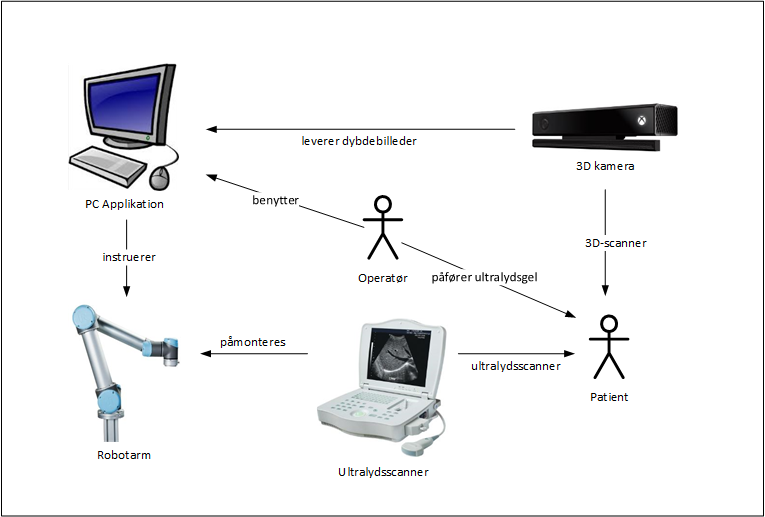
\includegraphics[width=0.50\textwidth]{figurer/d/Systembeskrivelse}
    \caption{Systembeskrivelse.}
    \label{Systembeskrivelse}
\end{figure}

\section{Aktører}
Aktørerne kan enten påvirke eller blive påvirket af systemet. De primære aktøre pårvirker systemet, mens de sekundere aktører bliver påvirket af systemet. Nedenfor ses et aktør-kontaktsdiagram, her er de primære aktøre afbilledet på venstre side af systemet og de sekundere er afbilledet på højre side af systemet. 

%%%
\subsection{Aktør-kontekstdiagram}
\begin{figure}[H]
    \centering
    \includegraphics[width=0.50\textwidth]{figurer/d/Aktor}
    \caption{Aktør-kontekstdiagram.}
    \label{akDiagram}
\end{figure}

%%%
\subsection{Aktørbeskrivelse}
\begin{longtabu} to \linewidth{@{}>{\sffamily}r *{2}{>{\sffamily}X[j]} >{\sffamily}l@{}}
    Aktørnavn &  Type &  Beskrivelse\\[-1ex]
    \midrule
   Operatør &  Primær &   Operatøren interagere med systemet, gennem et interface. \\
    Patient &  Sekundær &    Systemet foretager scanninger på Patienten. \\
   Ultralydsscanner & Sekundær &    Ultralydsscanneren bliver styret gennem systemt, til at lave ultralydsscanninger på patienten.\\
   3D kamera &  Sekundær &    3D kameraet skanner og detekterer det område hvor ultralydsscanneren til foretage sin skanning. \\
    Robotarm &   Sekundær &    Robotarmen styrer ultralydsscanneren i det detekterede område.\\
\label{actortable}
\end{longtabu}

%%%%%
\section{Ikke-funktionelle krav}\label{sect_IkFunk}
Ikke-funktionelle krav er begrænsninger til løsning af projektets funktionelle krav. Til at beskrive de ikke-funktionelle krav er MoSCoW og FURPS+ metoderne anvendt. 
MoSCoW-metoden betegner krav, som systemet skal opfylde (must), de krav som systemet bør realisere (should), de krav som systemet kunne realisere, men ikke har indvirkning på de andre krav (could), og de krav som omhandler fremtidige opdateringer og udvidelser (would).
  
FURPS+ står for:
\begin{enumerate}
 \item[F.] funktionelle krav, som er angivet i Use Cases.
\item[U.] Usability
\item[R.] Reliability
\item[P.] Performance 
\item[S.] Supportability 
\item[+.] ekstra krav til systemet, som ikke hører ind under ovenstående. 
\end{enumerate}

%%%
\subsection{Usability}
\begin{enumerate}
    \item[U1.] En operatør med kendskab til ultralyd skal kunne benytte systemet(must).
    \item[U2.] System bør have en brugervejledning (should). 
    \item[U3.] System skal have et interface (must).  
    \item[U4.] Operatør skal kunne vælge at scanne brystområde med 3D kamera (must). 
    \item[U5.] Operatør skal kunne ultralydsscanne en patient med robotarmen (must).  
\end{enumerate}

%%%
\subsection{Reliability}
\begin{enumerate}
    \item[R1.] 
\end{enumerate}

%%%
\subsection{Performance}
\begin{enumerate}
    \item[P1.] Scanningen med 3D kameraet og ultralydsscanning må max tage 10 minutter til sammen.  
    \item[P2.]  Startoptid skal være max 30 sekunder?
    \item[P3.] Svartid skal være max 1 sekund ved tryk på en vilkårlig knap. 
    \item[P4.] 3D kameraet må max være 1 minut om at tage 3D billedet. 
    \item[P5.] System skal max være 1 minut om at færdiggøre koordinater og positioner til robotarm. 
    \item[P6.] System skal benytte n tier architecture. 
    \item[P7.] Softwaren skal opbygges efter programmeringsprincipperne SOLID. 
    \item[P8.] Ultralydsscannerens opløsning skal minimum være ???. 
    \item[P9.] Tryksensoren skal kunne registrere et trykforskel på ???.
\end{enumerate}

%%%
\subsection{Supportability}
\begin{enumerate}
    \item[S1.] Systemets overflade skal kunne rengøres med en fugtig klud (must). 
    \item[S2.] Ultralydsscannerens probe skal kunne desinficeres med hospitalssprit (must). 
    \item[S3.] Ledninger til og fra hardwaren skal kunne opretholde deres funktionalitet på trods af et pludseligt træk (must). 
    \item[S4.] Operatør bør have mulighed for at skifte ultralydsscanner til systemet (sould).  
    \item[S5.] Operatør bør ikke have mulighed for at skifte komponenter i softwaren (sould).   
\end{enumerate}

%%%
\subsection{Ekstra(+)}\label{andrePlus}

\subsubsection{Brugssituationer}
\begin{enumerate}
    \item[+1.] I fremtiden kan System opdateres med en funktion, der lokaliserer knuder og identificerer knuder (would).
    \item[+2.] I fremtiden kan Operatør registrere en patient i system (would). 
    \item[+3.] I fremtiden kan Operatør gemme og hente en måling i system (would).  
    \item[+4.] I fremtiden kan Operatør slette en måling i system (would). 
    \item[+5.] I fremtiden kan System have en database, til at lagre data (would).
\end{enumerate}

%%%%%
\section{Funktionelle krav}\label{afsFunk}
De funktionelle krav er funktioner som systemet kan kunne. De funktionelle krav er beskrevet med use cases. 

%%%
\subsection{Use case-diagram}
\begin{figure}[H]
    \centering
    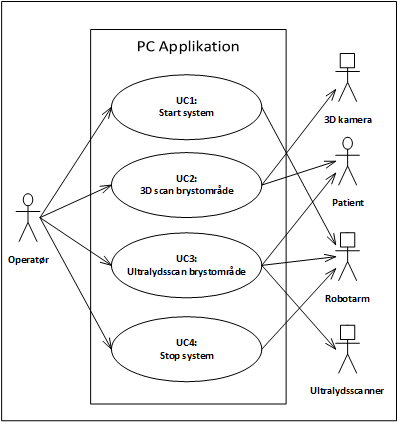
\includegraphics[width=0.50\textwidth]{figurer/d/UseCaseDiagram}
    \caption{Use Case Diagram.}
    \label{UseCaseDiagram}
\end{figure}

\section{Fully-dressed Use Cases}
%%%
\pagebreak
\subsection{Use Case 1}
\begin{tabular}{ | l | p{0.8\textwidth} | }
  \hline
  \multicolumn{2}{|c|}{\textbf{UC1: Start System}} \\ \hline
  \textbf{Goal} & To initiate the system and prepare to scan  \\ \hline
  \textbf{Initiation} & Operator opens the software on the computer.  \\ \hline
  \textbf{Precondition} & The computer has been booted  \\ \hline
  \textbf{Postcondition} & The software has activated Robot arm, 3D camera and Ultrasound scanner.  \\ \hline
  \textbf{Main Scenario} & 
  	{\begin{enumerate} 
  	\item Operator starts System
  	\end{enumerate}} \\ \hline
  \textbf{Exceptions} & \hspace{1cm} \\ \hline
\end{tabular}

%%%

\subsection{Use Case 2}
\begin{tabular}{ | l | p{0.8\textwidth} | }
  \hline
  \multicolumn{2}{|c|}{\textbf{UC2: Detect chest area}} \\ \hline
  \textbf{Goal} & To construct a depth image of Patient’s chest area, so that UC3 can be initiated  \\ \hline
  \textbf{Initiation} & Operator selects ’3D Scan’  \\ \hline
  \textbf{Precondition} & UC1 has been completed  \\ \hline
  \textbf{Postcondition} & Patient’s chest area has been scanned \\ \hline
  \textbf{Main Scenario} & 
  	{\begin{enumerate} 
  	\item 3D camera scans chest area
  	\item 3D camera feeds boundary points to System
  	\item Operator verifies depth image
  		\begin{itemize}
  		\item \textit{[Depth image is distorted]}
  		\end{itemize}
  	\end{enumerate}} \\ \hline
  \textbf{Exceptions} & 
  	{\begin{itemize} 
  	\item \textit{[Depth image is distorted]}
  		\begin{enumerate}
  		\item Enter UC2, item 1.
  		\end{enumerate}
  	\end{itemize}} \\ \hline
\end{tabular}

\subsection{Use Case 3}
\begin{tabular}{ | l | p{0.8\textwidth} | }
  \hline
  \multicolumn{2}{|c|}{\textbf{UC3: Detect chest area}} \\ \hline
  \textbf{Goal} & To perform a medical sonography of the chest area \\ \hline
  \textbf{Initiation} & Operator selects ‘Ultrasound Scan’ \\ \hline
  \textbf{Precondition} & UC2 has been completed \\ \hline
  \textbf{Postcondition} & System has instructed Robot arm to move Ultrasound scanner in order to construct a medical sonographic image of Patient’s chest area  \\ \hline
  \textbf{Main Scenario} & 
  	{\begin{enumerate} 
  	\item Operator starts Ultrasound scanner
  	\item Operator chooses 'Ultrasound Scan' in System
  	\item System utilizes depth image from UC2 to feed Robot arm positions and rotations in order to move Ultrasound scanner
  	\item System stops Robot arm
  		\begin{itemize}
  		\item \textit{[Operator stops Robot arm]}
  		\end{itemize}
  	\item Operator stops Ultrasound scanner
  	\end{enumerate}} \\ \hline
  \textbf{Exceptions} & 
  	{\begin{itemize} 
  	\item \textit{[Operator stops Robot arm]}
  		\begin{enumerate}
  		\item Operator chooses 'Stop Ultrasound Scan' in System.
  		\item System stops moving Robot arm prematurely.
  		\end{enumerate}
  	\end{itemize}} \\ \hline
\end{tabular}

\subsection{Use Case 4}
\begin{tabular}{ | l | p{0.8\textwidth} | }
  \hline
  \multicolumn{2}{|c|}{\textbf{UC4: Stop system}} \\ \hline
  \textbf{Goal} & To stop System \\ \hline
  \textbf{Initiation} & Operator \\ \hline
  \textbf{Precondition} & UC1 has been completed \\ \hline
  \textbf{Postcondition} & System has shut down  \\ \hline
  \textbf{Main Scenario} & 
  	{\begin{enumerate} 
  	\item Operator closes System software by hitting the Close button in the top right corner
  	\item Upon exit, Robot arm is set to default position
  	\item System shuts down
  	\end{enumerate}} \\ \hline
  \textbf{Exceptions} & \hspace{1cm} \\ \hline
\end{tabular}

\pagebreak
